\documentclass{beamer}

\mode<presentation>
{
  \usetheme{CambridgeUS}
  \usecolortheme{orchid}
  \setbeamercovered{transparent}
  \useinnertheme{rectangles}
  \setbeamertemplate{navigation symbols}{}
  \usefonttheme[onlymath]{serif}
  \setbeamercolor{title}{bg=alerted text.fg!85!black, fg=white}
  \setbeamercolor{item projected}{bg=alerted text.fg!85!black}
  \setbeamertemplate{enumerate items}[default]
  \setbeamercolor{local structure}{fg=alerted text.fg!85!black}
}

\usepackage[english]{babel}
\usepackage[utf8]{inputenc}
\usepackage[T1]{fontenc}
\usepackage{lmodern}
\usepackage{pifont}
\usepackage{booktabs}

\definecolor{hdblue}{HTML}{3366cc}
\hypersetup{colorlinks,linkcolor=,urlcolor=hdblue, citecolor=hdblue}

\usepackage{amsmath}
\usepackage{outlines}
\usepackage{caption}
\usepackage{natbib}

\usepackage{subcaption}
\usepackage{algorithm}
\usepackage{algorithmic}
\usepackage{amsmath,bm}

\newcommand{\xmark}{\ding{55}}
\newcommand{\highlight}[1]{%
  \colorbox{red!50}{$\displaystyle#1$}}
\newcommand{\blue}[1] {\textcolor{blue}{#1}}
\newcommand{\red}[1] {\textcolor{red}{#1}}

\title[Learning Graphical Models]{Learning to Discover Sparse Graphical Models}

% \subtitle
% {Presentation Subtitle} % (optional)

\author[Dogan]
{%
  \texorpdfstring{
    \vspace{-0.50cm}
    \begin{columns}
      \column{.55\linewidth}
      \centering
      ICML 2017 \citep{belilovsky2017learning}
    \end{columns}
    \vspace{0.1cm}
    \begin{columns}
      \column{.3\linewidth}
      \centering
      Eugene Belilovsky \\ \tiny{\textit{ESAT-PSI, KU Leuven} \\
        \textit{INRIA} \\ \textit{University of Paris-Saclay}}
      \column{.3\linewidth}
      \centering
      Kyle Kastner \\ \tiny{\textit{University of Montreal}}
    \end{columns}
    \vspace{0.1cm}
    \begin{columns}
      \column{.3\linewidth}
      \centering
      Gael Varoquaux \\ \tiny{\textit{INRIA}}
      \column{.3\linewidth}
      \centering
      Matthew B. Blaschko \\ \tiny{\textit{ESAT-PSI, KU Leuven}}
    \end{columns}
    \vspace{0.1cm}
    \begin{columns}
      \column{.45\linewidth}
      \centering
      Presented by:\\
      Haluk Dogan\\
      \url{https://haluk.github.io/}\\
      \href{mailto:hlk.dogan@gmail.com}{hlk.dogan@gmail.com}
    \end{columns}
}
{Dogan}
}

\institute[UNL] % (optional, but mostly needed)
{
  Department of Computer Science\\
  University of Nebraska-Lincoln
}

\date[\today] % (optional)
{\today}

\subject{Talks}

\pgfdeclareimage[height=0.5cm]{university-logo}{img/logo}
\logo{\pgfuseimage{university-logo}}

\begin{document}

\begin{frame}
  \titlepage
\end{frame}

\section{Introduction}
\subsection{Graphical Models}
\begin{frame}{Graphical Models}
  \begin{columns}
    \begin{column}{0.32\textwidth}
      \begin{figure}[ht]
        \centering
        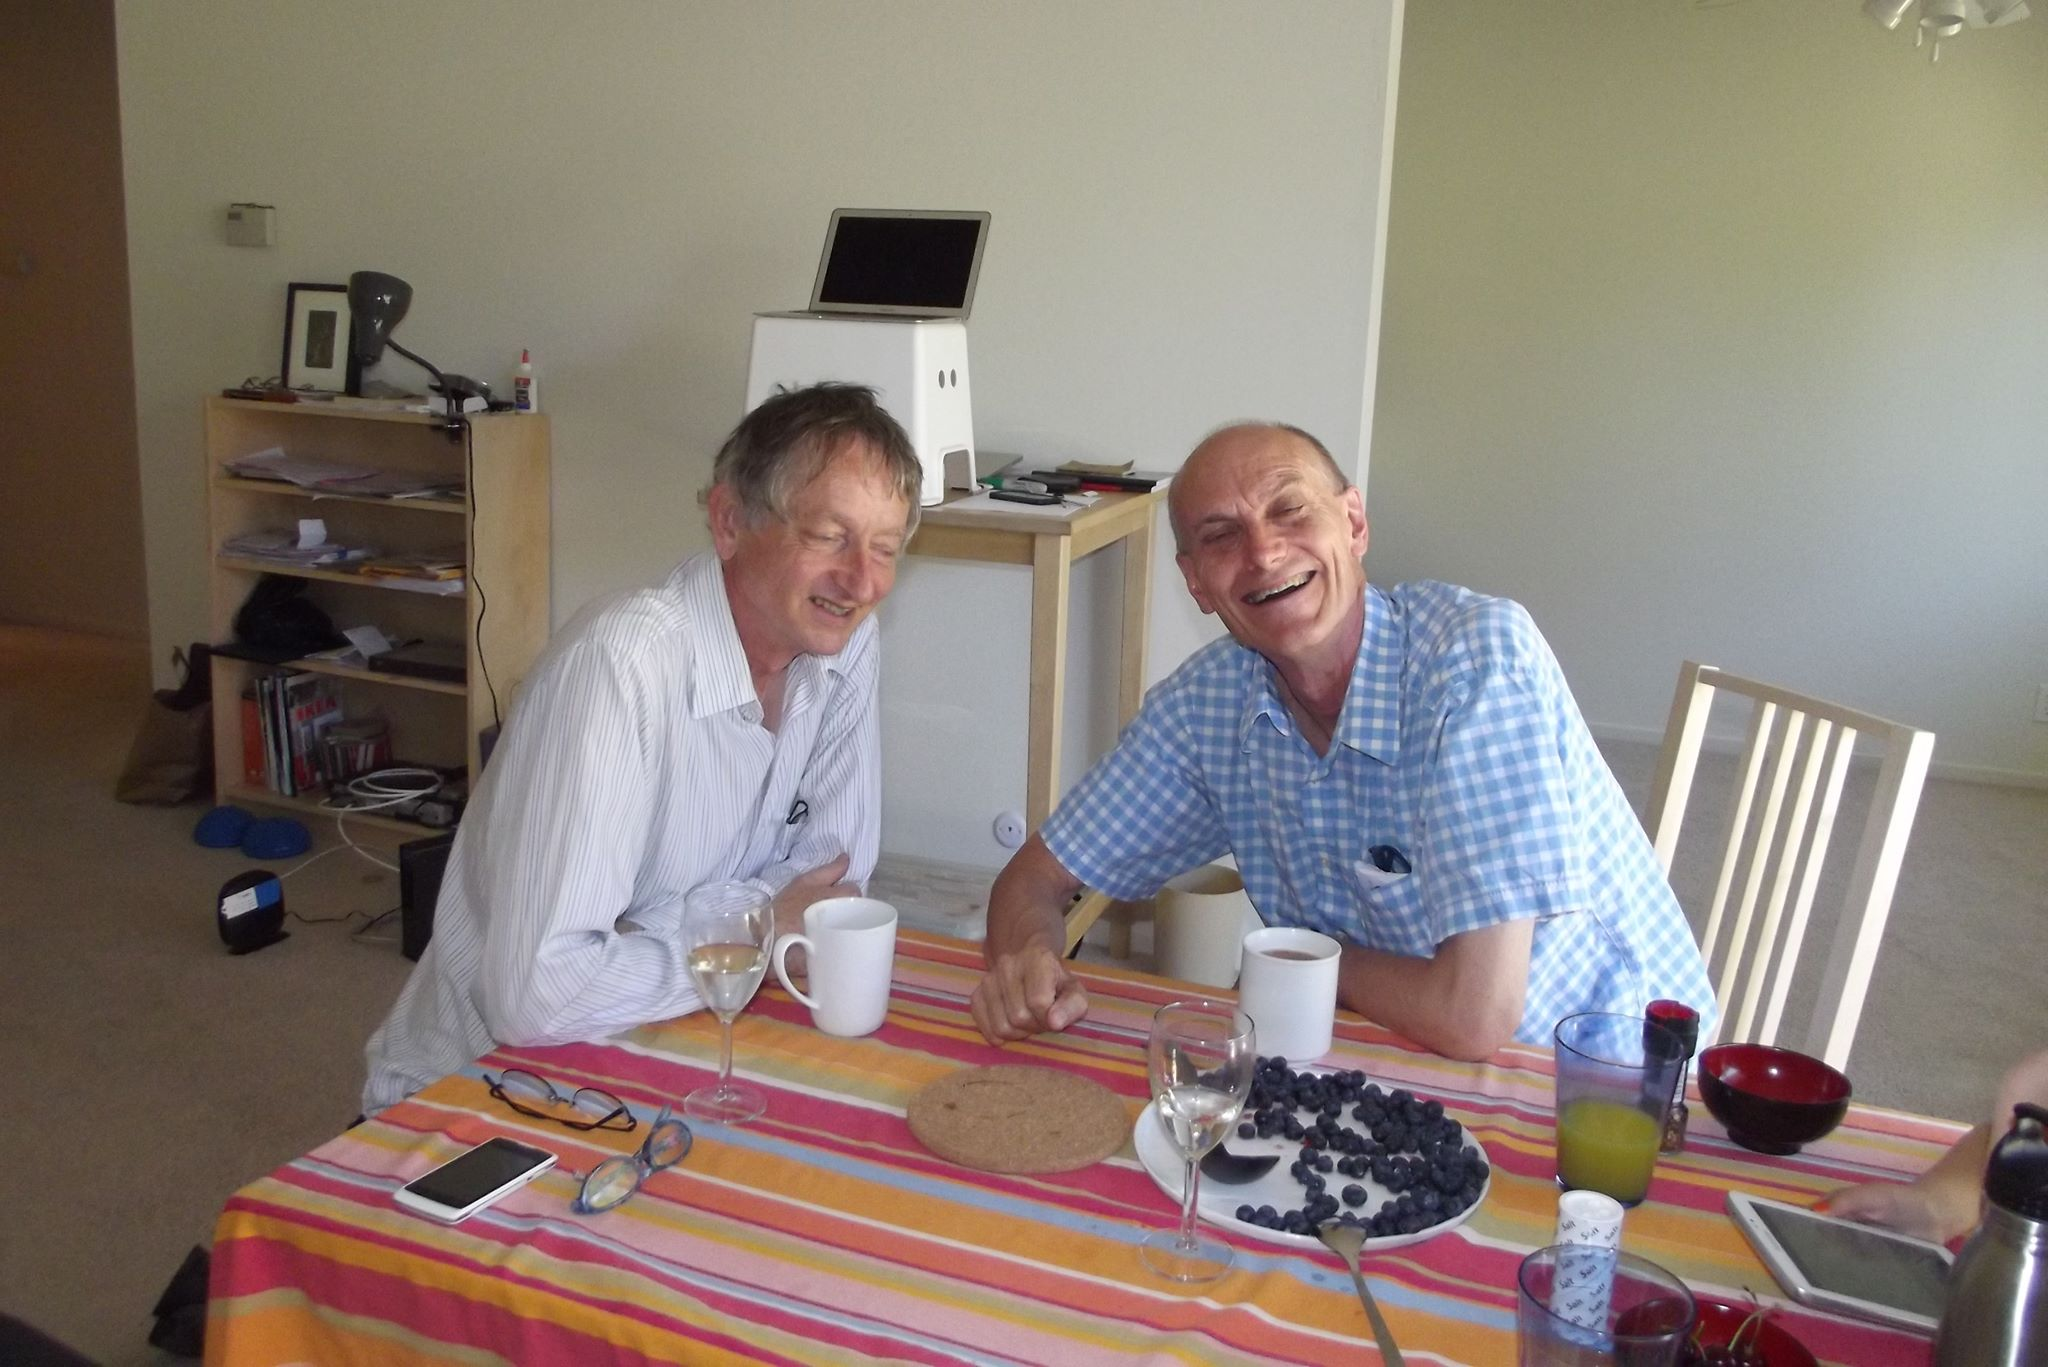
\includegraphics[width=1\textwidth,height=0.5\textheight]{img/hinton_chris}
        \caption*{\tiny{Geoffrey Hinton and Chris Stephenson\label{fig:hinton-chris}}}
      \end{figure}
    \end{column}
    \begin{column}{0.32\textwidth}
      \begin{figure}[ht]
        \centering
        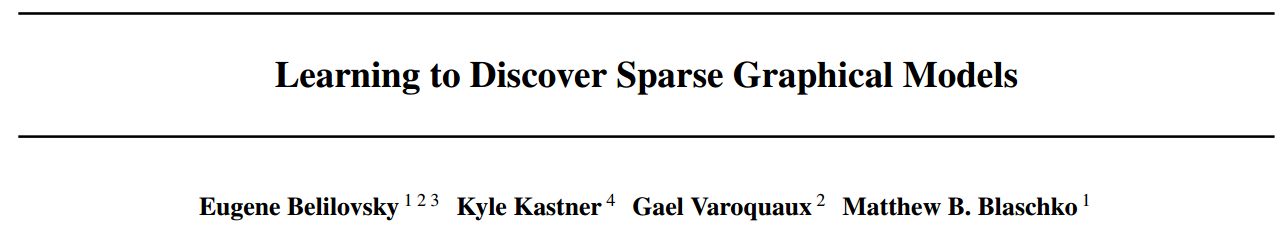
\includegraphics[width=1\textwidth,height=0.2\textheight]{img/learning_graphical_models}
        \caption*{\label{fig:snapshot}}
      \end{figure}
    \end{column}
    \begin{column}{0.32\textwidth}
      \begin{figure}[ht]
        \centering
        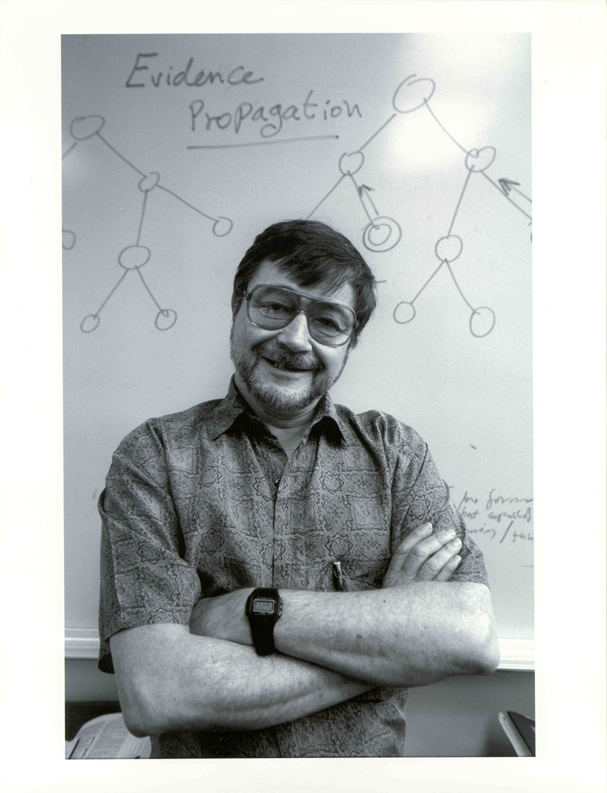
\includegraphics[width=1\textwidth,keepaspectratio]{img/judea_pearl}
        \caption*{\tiny{Judea Pearl\label{fig:judea-pearl}}}
      \end{figure}
    \end{column}
  \end{columns}
\end{frame}

\begin{frame}{Graphical Models (cont'd)}
  \begin{figure}[ht]
    \centering
    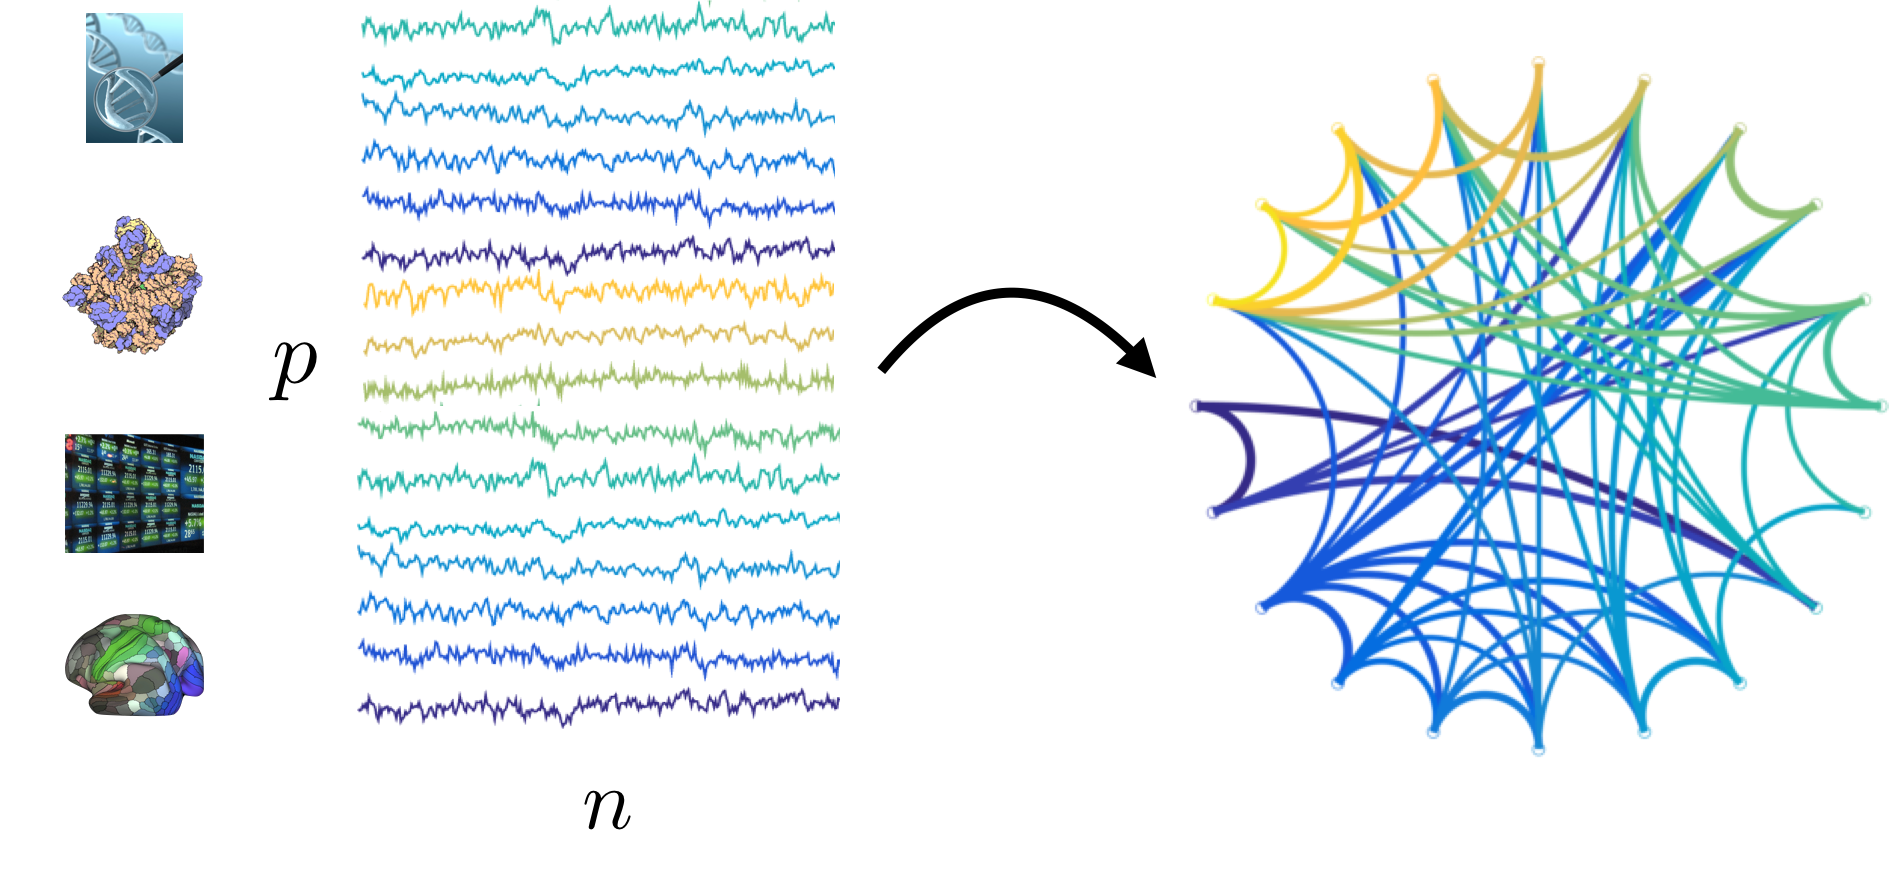
\includegraphics[width=1\textwidth,keepaspectratio]{img/skggm_network}
    \caption*{\label{fig:network}}
  \end{figure}
\end{frame}

\begin{frame}<beamer>{Outline}
    \tableofcontents[currentsection,currentsubsection]
\end{frame}

\begin{frame}{Preliminaries for Gaussian Graphical Models}
  \begin{itemize}
  \item $X=[X_1,X_2,\dots,X_p]$ and $X \sim N(\mu, \mathbf{\Sigma})$
  \item $p ( X ; \mu , \mathbf{\Sigma} ) = \frac { 1 } { ( 2 \pi ) ^ { p / 2 }
      | \mathbf{\Sigma} | ^ { 1 / 2 } } \exp \left( - \frac { 1 } { 2 } ( x -
      \mu ) ^ { T } \mathbf{\Sigma} ^ { - 1 } ( x - \mu ) \right)$
  \item Mean $\mu \in \mathbf { \mathbb{R} } ^ { p }$
  \item Covariance matrix $\mathbf{\Sigma} \in \mathbf { \mathbb{S} } _ { + + } ^ { p }$
  \item Precision matrix $\Theta = \mathbf{\Sigma}^{-1}$
  \end{itemize}
  \begin{columns}
    \begin{column}{0.38\textwidth}
      \begin{figure}[ht]
        \centering
        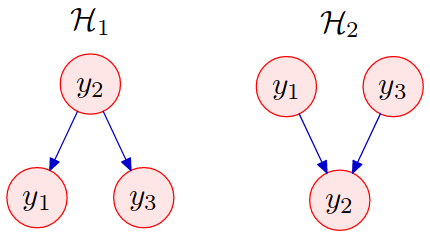
\includegraphics[width=1\textwidth,keepaspectratio]{img/belief}
        \caption*{Belief Network\label{fig:belief}\footnotemark}
      \end{figure}
    \end{column}
    \begin{column}{0.48\textwidth}
      \[
        \stackrel{\mbox{A}}{%
          \begin{bmatrix}
            9 & 3 & 1 \\
            3 & 9 & 3 \\
            1 & 3 & 9
          \end{bmatrix}%
        } \quad
        \stackrel{\mbox{B}}{%
          \begin{bmatrix}
            8 & -3 & 1 \\
            -3 & 9 & -3 \\
            1 & -3 & 8
          \end{bmatrix}%
        }
      \]
      \[
        \stackrel{\mbox{C}}{%
          \begin{bmatrix}
            9 & 3 & 0 \\
            3 & 9 & 3 \\
            0 & 3 & 9
          \end{bmatrix}%
        } \quad
        \stackrel{\mbox{D}}{%
          \begin{bmatrix}
            9 & -3 & 0 \\
            -3 & 10 & -3 \\
            0 & -3 & 9
          \end{bmatrix}%
        }
      \]
    \end{column}
  \end{columns}
  \footnotetext{\tiny{``The Humble Gaussian Distribution'' by David MacKay}}
\end{frame}
\begin{frame}{Graphical Lasso}
  \begin{itemize}
  \item $\mathbf { X } _ { n \times p }$, $\mu=0^p$ and $\mathbf{\Sigma} \in
    \mathbf { \mathbb{S} } _ { + + } ^ { p }$
  \item Our task is to estimate $\mathbf{\Sigma}$
    \begin{itemize}
    \item Challenging problem when $n \ll p$
    \item Ordinary MLE does not exits
      \begin{itemize}
      \item Poorly behaved
      \item Regularization is needed ($\ell _ { 1 }$ norm)
      \end{itemize}
    \item Assumption: $\Theta = \mathbf{\Sigma} ^ { - 1 }$ is sparse
    \end{itemize}
  \end{itemize}
  \begin{block}{Objective Function}
    \[
      f _ { g l } ( \hat { \boldsymbol { \Sigma } } ) = \arg \min _ { \mathbf { \Theta } \succ 0 } - \log | \Theta | + \operatorname { Tr } ( \hat { \mathbf { \Sigma } } \Theta ) + \lambda \| \Theta \| _ { 1 }
    \]
  \end{block}
\end{frame}
\begin{frame}{Graphical Lasso (cont'd)}
  Why do we put sparsity constraint?
  \begin{itemize}
  \item $\mathbf{\Sigma}$ is $p \times p$ matrix
  \item Estimating $\mathbf{\Sigma}$ requires $O(p^2)$ measurements
  \item Each observation $X_i \in \mathbb{R}^p$ provides $p$ scalar
    values. $O(p)$ is not enough to estimate $\mathbf{\Sigma}$
  \item Sparse graphical model:
    \begin{itemize}
    \item $|E| \ll O(p^2)$
    \item Suppose each vertex (variable) is connected to at most $d
      \ll p$ other vertices, there are only $O(dp)$ edges in the graph
    \end{itemize}
  \end{itemize}
\end{frame}
\begin{frame}{Graphical Lasso (cont'd)}
  Alternative penalties:
  \begin{itemize}
    \item Fused graphical lasso, Group graphical lasso
      \citep{danaher2014joint}
    \item Elastic net penalty (combines $\ell_1$ and $\ell_2$)
      \citep{ryali2012estimation}
    \item Mixed norm $\ell_{21}$ \citep{varoquaux2010brain}
  \end{itemize}
  Challenges:
  \begin{itemize}
    \item Novel surrogates for structured-sparsity assumptions on MRF
      structures
    \item Priors need to be formulated
    \item Regularization parameters are often unintuitive
      \begin{itemize}
        \item Model selection becomes difficult
      \end{itemize}
  \end{itemize}
\end{frame}
\begin{frame}{Proposed Approach}
  \begin{itemize}
  \item Learn the estimator
    \begin{itemize}
    \item Select a function from a large flexible function class
      by risk minimization for edge estimation
    \end{itemize}
  \item Sampling from a distribution of graphs and empirical
    covariances with desired properties
  \item Polynomial function
    \begin{itemize}
    \item Neural network
    \item Function class is CNN
    \end{itemize}
  \end{itemize}
\end{frame}

\section{Learning the Estimator}
\begin{frame}{Learning the Estimator}
  \begin{itemize}
  \item $\mathbf{X} \in \mathbb{R}^{n \times p}$
  \item $G=(V,E)$ be an undirected and unweighted graph
  \item $\mathcal{L}=\{0,1\}$ and $N_e=\frac{p(p-1)}{2}$ the maximum
    possible edges
  \item $Y^{ij} =  \begin{cases}
      0 &  x_i  \perp x_j | x_{V\backslash{i,j}} \\
      1 & x_i  \not\perp x_j | x_{V\backslash{i,j}} .
    \end{cases}$
  \item $\hat{Y}=g_{w}(\mathbf{X})$ is an approximate structure
    discovery method
    \begin{itemize}
      \item $\hat{\mathbf{\Sigma}}$: $g_{w}(\mathbf{X}) := f_{w}(\hat{\mathbf{\Sigma}})$
      \end{itemize}
    \item We want to minimize expected risk: $R ( f ) = \mathbb { E }
      _ { ( \hat { \mathbf { \Sigma } } , Y ) \sim \mathbb { P } } [ l
      ( f ( \hat { \mathbf { \Sigma } } ) , Y ) ]$
      \begin{itemize}
        \item $\mathbb { P }$ on $\mathbb { R } ^ { p \times p }
          \times \mathcal { L } ^ { N _ { e } }$
        \item $l : \mathcal { L } ^ { N _ { e } } \times \mathcal { L }
          ^ { N _ { e } } \rightarrow \mathbb { R } ^ { + }$ ($0/1$
          loss function)
      \end{itemize}
  \end{itemize}
\end{frame}
\begin{frame}{Learning the Estimator (cont'd)}
  \begin{itemize}
  \item Distribution $\mathbb{P}$ may not be tractable:
  \item Empirical risk minimization:
    \begin{itemize}
      \item $N$ samples $\{Y_k,\mathbf{\Sigma}_k \}_{k=1}^N$ drawn
        from $\mathbb{P}$
      \item $\min\limits_{w} \frac{1}{N}\sum_{k=1}^N
        l(f_{w}(\mathbf{\hat{{\Sigma}}}_k),Y_k)$
      \item $\hat{l}: \mathbb{R}^{N_e} \times \mathcal{L}^{N_e}$
        \begin{itemize}
        \item 0/1 loss is not convex
        \item $\sum\limits_{i \neq j} \big( Y^{ij}\log (f_{w}^{ij}(\hat{\mathbf{\Sigma}}))+(1-Y^{ij})\log (1-f_{w}^{ij}(\hat{\mathbf{\Sigma}}))\big) .$
        \end{itemize}
    \end{itemize}
  \end{itemize}
  \scalebox{0.75}{
    \begin{minipage}{0.7\linewidth}
      \begin{algorithm}[H]
        \begin{algorithmic}
          \footnotesize
          \caption{\small Training a GGM edge estimator}\label{alg:struct}
          \FOR{i $\in \{1,..,N \}$}
          \STATE Sample $G_i \sim \mathbb{P}(G)$
          \STATE Sample $\mathbf{\Theta}_i \sim \mathbb{P}(\mathbf{\Theta}|G=G_i)$
          \STATE $\mathbf{X}_i \leftarrow \{x_j\sim N(0,\mathbf{\Theta}_i^{-1}) \}_{j=1}^n$
          \STATE Construct $(Y_i,\mathbf{\hat{\Sigma}}_i)$ pair from $(G_i,\mathbf{X_i})$
          \ENDFOR
          \STATE Select Function Class $\mathcal{F}$ (e.g. CNN)
          \STATE Optimize: $\min\limits_{f \in \mathcal{F}} \frac{1}{N}\sum_{k=1}^N \hat{l}(f(\mathbf{\hat{{\Sigma}}}_k),Y_k))$
        \end{algorithmic}
      \end{algorithm}
    \end{minipage}
    }
\end{frame}
\begin{frame}{Neural Network Graph Estimator}
  \begin{itemize}
    \item If the data is standardized, each entry of $\mathbf{\Sigma}$
      corresponds to the correlation $\rho_{i,j}$
    \item $d$th-order partial correlation can be obtained from
      $(d-1)$th-order partial correlation
      \[
        \rho ( i , j | \mathbf { Z } ) = \frac { \rho ( i , j | \mathbf { Z } \backslash \left\{ z _ { 0 } \right\} ) - \rho \left( i , z _ { 0 } | \mathbf { Z } \backslash \left\{ z _ { 0 } \right\} \right) \rho \left( j , z _ { 0 } | \mathbf { Z } \backslash \left\{ z _ { 0 } \right\} \right) } { \sqrt { \left( 1 - \rho ^ { 2 } \left( i , z _ { 0 } | \mathbf { Z } \backslash \left\{ z _ { 0 } \right\} \right) \left( 1 - \rho ^ { 2 } \left( j , z _ { 0 } | \mathbf { Z } \backslash \left\{ z _ { 0 } \right\} \right) \right) \right. } }
      \]
      \[
        \rho_{i,j|\mathbf{Z}}=(\rho_{i,j|\mathbf{Z}\backslash{z_o}}-\rho_{i,z_o|\mathbf{Z}\backslash{z_o}}\rho_{j,z_o|\mathbf{Z}\backslash{z_o}})\frac{1}{D}
      \]
    \end{itemize}
    \begin{block}{}
      Using gradient descent, a neural network with only two layers can learn a polynomial function of degree $d$ to arbitrary precision given sufficient hidden units \citep{andoni2014learning}
    \end{block}
\end{frame}
\begin{frame}{Neural Network Graph Estimator (cont'd)}
  \begin{itemize}
    \item DP can yield polynomial computation time and require only low order polynomial computations
  \end{itemize}
  \begin{figure}[ht]
    \centering
    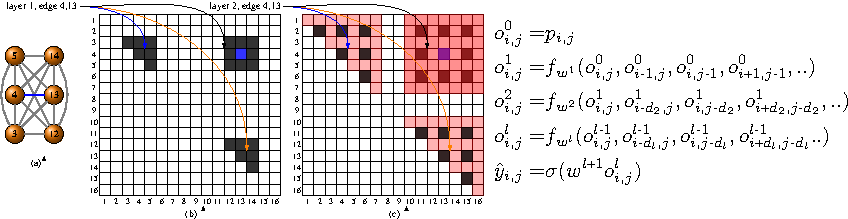
\includegraphics[width=1\textwidth,keepaspectratio]{img/dnet}
    \caption*{\label{fig:dnet}}
  \end{figure}
  \vspace{-1cm}
  \begin{figure}[ht]
    \centering
    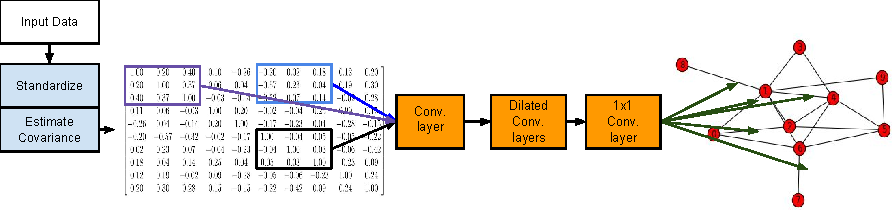
\includegraphics[width=0.8\textwidth,keepaspectratio]{img/workflow}
    \caption*{\label{fig:workflow}}
  \end{figure}
\end{frame}
\section{Experiments}
\begin{frame}{Experiments}
\begin{table}[h]
\begin{center}
\resizebox{0.7\columnwidth}{!}{
\begin{tabular}{ |c|c|c|c|c| }
\hline
Experimental Setup	&	Method	&	Prec@$5\%$	&	AUC	&	 CE       \\\hline
 & Glasso & 0.361 $\pm$ 0.011 & 0.624 $\pm$ 0.006  & 0.07  \\
Gaussian& Glasso (optimal) & 0.384 $\pm$ 0.011 & 0.639 $\pm$ 0.007  & 0.07 \\
 Random Graphs& BDGraph & 0.441 $\pm$ 0.011 & 0.715 $\pm$ 0.007  & 0.28 \\
($n=35,p=39$)& DeepGraph-39 & 0.463 $\pm$ 0.009 & 0.738 $\pm$ 0.006  & $0.07$ \\
& DeepGraph-39+Perm & \bm{$0.487 \pm 0.010$} & \bm{$0.740 \pm 0.007$}  & 0.07 \\    \hline
& Glasso & 0.539 $\pm$ 0.014 & 0.696 $\pm$ 0.006  & 0.07\\
Gaussian& Glasso (optimal) & 0.571 $\pm$ 0.011 & 0.704 $\pm$ 0.006  & 0.07\\
 Random Graphs& BDGraph & \bm{$0.648 \pm 0.012$} &\bm{ $0.776 \pm 0.007$}  & 0.16\\
($n=100,p=39$)& DeepGraph-39 & 0.567 $\pm$ 0.009 & 0.759 $\pm$ 0.006  & 0.07 \\
& DeepGraph-39+Perm & $0.581 \pm 0.008$ & $0.771 \pm 0.006$  & 0.07 \\\hline
& Glasso & 0.233 $\pm$ 0.010 & 0.566 $\pm$ 0.004  & 0.07 \\
Gaussian & Glasso (optimal) & 0.263 $\pm$ 0.010 & 0.578 $\pm$ 0.004  & 0.07  \\
Random Graphs& BDGraph & 0.261 $\pm$ 0.009 & 0.630 $\pm$ 0.007  & 0.41 \\
($n=15,p=39$)& DeepGraph-39 & 0.326 $\pm$ 0.009 & 0.664 $\pm$ 0.008  & 0.08 \\
& DeepGraph-39+Perm &\bm{$0.360 \pm 0.010$} & \bm{$0.672 \pm 0.008$}  & 0.08 \\\hline

	& Glasso & 0.312 $\pm$ 0.012 & 0.605 $\pm$ 0.006  & 0.07  \\
Laplace & Glasso (optimal) & 0.337 $\pm$ 0.011 & 0.622 $\pm$ 0.006  & 0.07 \\
Random Graphs& BDGraph & 0.298 $\pm$ 0.009 & 0.687 $\pm$ 0.007  & 0.36 \\
($n=35,p=39$)& DeepGraph-39 & 0.415 $\pm$ 0.010 & 0.711 $\pm$ 0.007  & 0.07  \\
& DeepGraph-39+Perm &\bm{$0.445 \pm 0.011$} & \bm{$0.717 \pm 0.007$}  & 0.07  \\\hline
%& Glasso & 0.219 $\pm$ 0.011 & 0.613 $\pm$ 0.007  & 0.055 $\pm$ 0.000 \\
%& Glasso (optimal) & 0.222 $\pm$ 0.011 & 0.618 $\pm$ 0.007  & 0.056 $\pm$ 0.000 \\
%Gaussian Hub Graphs& BDGraph & 0.288 $\pm$ 0.007 & 0.728 $\pm$ 0.005  & 0.280 $\pm$ 0.006 \\
%(n=35)& DeepGraph-39 & 0.279 $\pm$ 0.006 & 0.742 $\pm$ 0.005  & 0.060 $\pm$ 0.000 \\
%& DeepGraph-39+Perm & 0.338 $\pm$ 0.006 & 0.772 $\pm$ 0.005  & 0.061 $\pm$ 0.000 \\\hline
& Glasso & 0.387 $\pm$ 0.012 & 0.588 $\pm$ 0.004  & 0.11 \\
Gaussian& Glasso (optimal) & 0.453 $\pm$ 0.008 & 0.640 $\pm$ 0.004  & 0.11 \\
Small-World Graphs & BDGraph & 0.428 $\pm$ 0.007 & 0.691 $\pm$ 0.003  & 0.17 \\
(n=35,p=39)& DeepGraph-39 & \bm{$0.479 \pm 0.007$} & 0.709 $\pm$ 0.003  & 0.11\\
& DeepGraph-39+Perm & 0.453 $\pm$ 0.007 & \bm{$0.712 \pm 0.003$}  & 0.11	\\\cline{2-5}
& DeepGraph-39+update & \bm{$0.560 \pm 0.008$} & \bm{$0.821 \pm 0.002$}  & 0.11 \\
& DeepGraph-39+update+Perm & 0.555 $\pm$ 0.007 & 0.805 $\pm$ 0.003  & 0.11 \\\hline
\end{tabular}
}
\end{center}
\end{table}
\end{frame}
\begin{frame}{Experiments (cont'd)}

\captionsetup{type=table}
\resizebox{1\columnwidth}{!}{
\begin{tabular}{ |c|c|c|c|c| }
\hline
Method	&Prec@$0.05\%$ &	Prec@$5\%$	&	AUC	&	 CE       \\\hline


 random &0.052 $\pm$ 0.002 &  0.053 $\pm$ 0.000  & 0.500 $\pm$ 0.000  & 0.05 \\
 Glasso &0.156 $\pm$ 0.010  &0.055 $\pm$ 0.001  & 0.501 $\pm$ 0.000  & 0.05 \\
 Glasso (optimal) &0.162 $\pm$ 0.010  &0.055 $\pm$ 0.001 & 0.501 $\pm$ 0.000  & 0.05 \\
 DeepGraph-500 &0.449 $\pm$ 0.018 & 0.109 $\pm$ 0.002 & 0.543 $\pm$ 0.002  & 0.06 \\
 DeepGraph-500+Perm &$\bm{0.583 \pm 0.018}$  &$\bm{0.116 \pm 0.00}$2  & \bm{$0.547 \pm 0.002$}  & \bm{$0.06$} \\\hline
\end{tabular}
}

\vspace{1cm}

\begin{tabular}{ |c|c|c| }
 \hline
  			  			 & 50 nodes (s) & 500 nodes (s)  \\
  			  			 \hline
 \texttt{sklearn} GraphLassoCV & 4.81 & 554.7\\
 \texttt{BDgraph}     & 42.13  & N/A\\
 DeepGraph & \textbf{\textit{0.27}} & \textbf{\textit{5.6}}\\
 \hline
\end{tabular}
\end{frame}

\begin{frame}{Experiments (cont'd)}
  \begin{columns}
    \begin{column}{0.48\textwidth}
      \begin{figure}[ht]
        \centering
        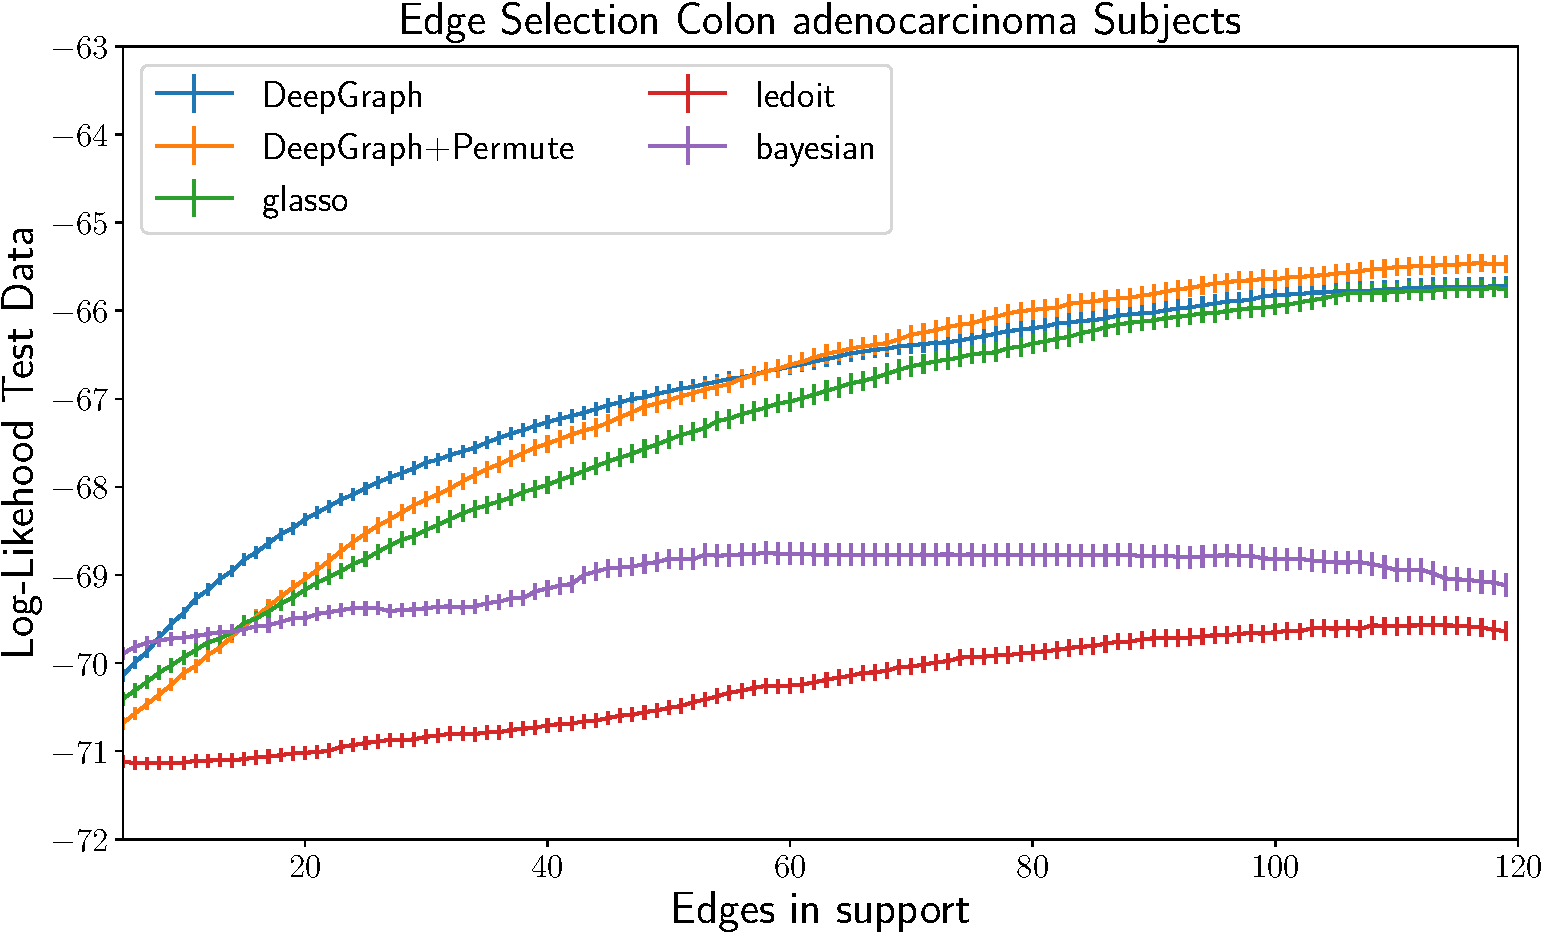
\includegraphics[width=1\textwidth,keepaspectratio]{img/New_Gene_COAD_nsamps_40_repetitions_150_errorbar_1-crop}
      \end{figure}
    \end{column}
    \begin{column}{0.48\textwidth}
      \begin{figure}[ht]
        \centering
        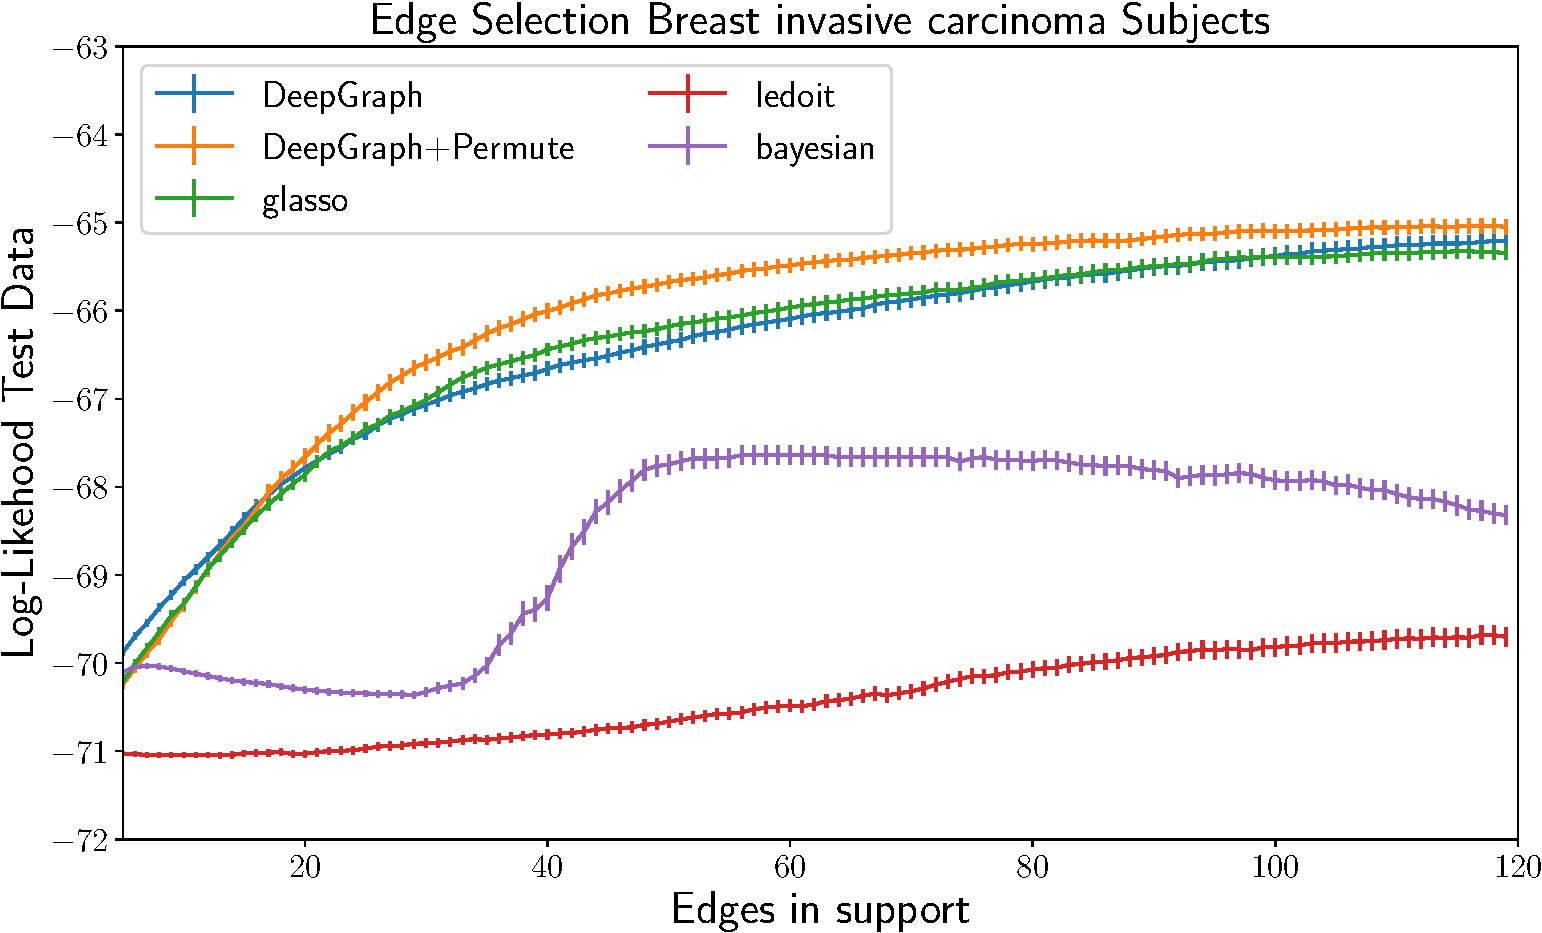
\includegraphics[width=1\textwidth,keepaspectratio]{img/New_Gene_BRCA_nsamps_40_repetitions_150_errorbar_1-crop}
      \end{figure}
    \end{column}
  \end{columns}
  \begin{columns}
    \begin{column}{0.48\textwidth}
      \begin{figure}[ht]
        \centering
        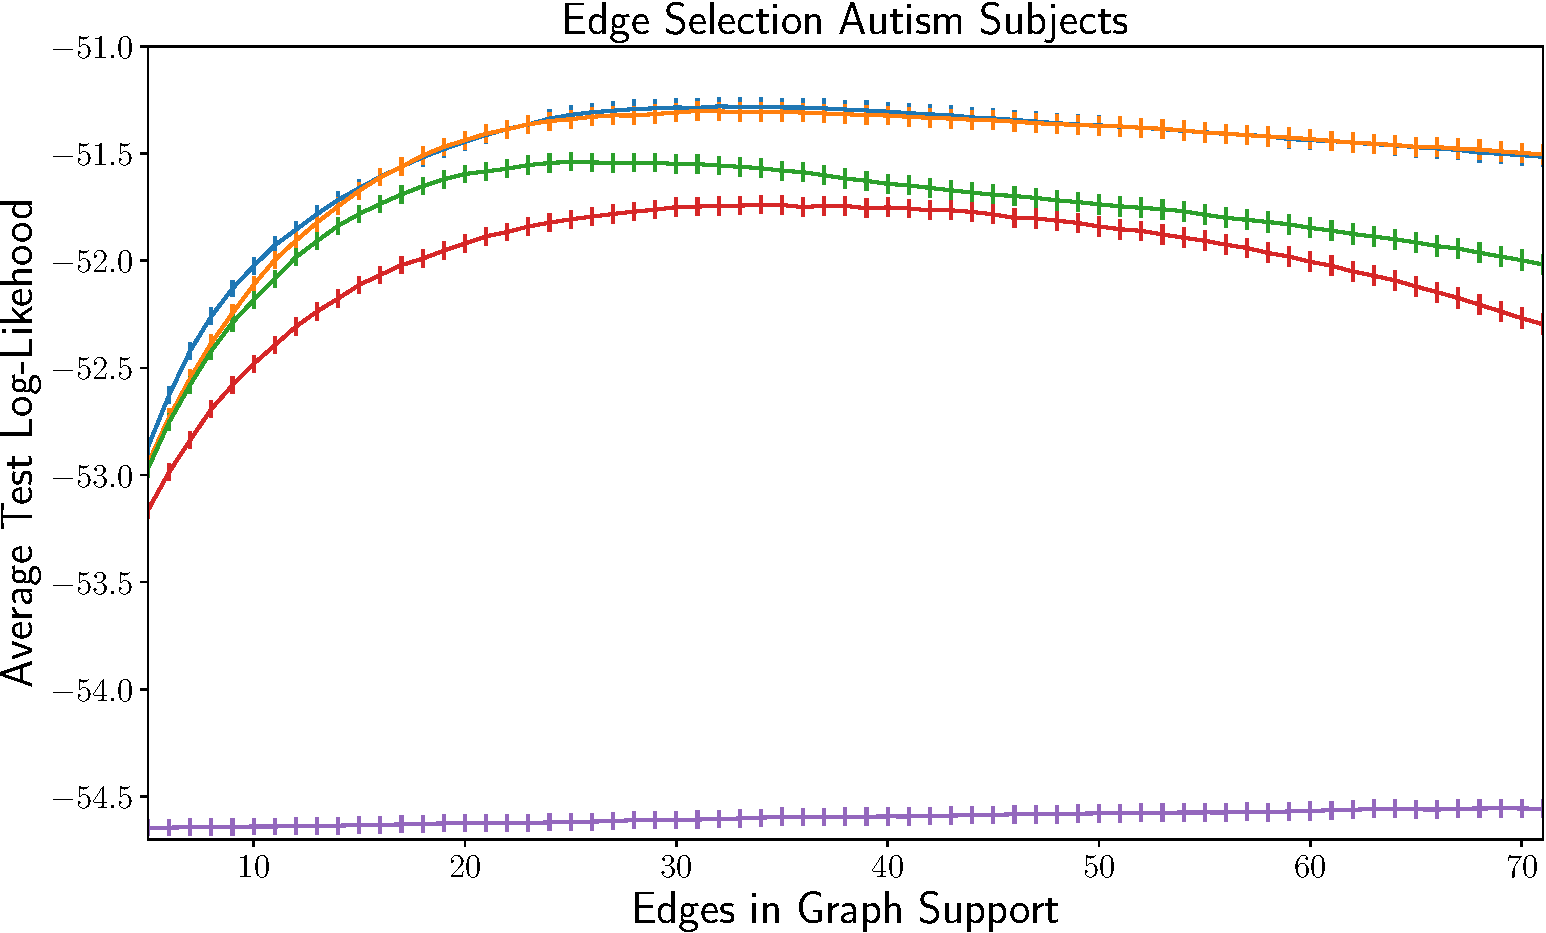
\includegraphics[width=1\textwidth,keepaspectratio]{img/New_ABIDE_Autism_nsamps_35_repetitions_1479_errobar_1-crop}
      \end{figure}
    \end{column}
    \begin{column}{0.48\textwidth}
      \begin{figure}[ht]
        \centering
        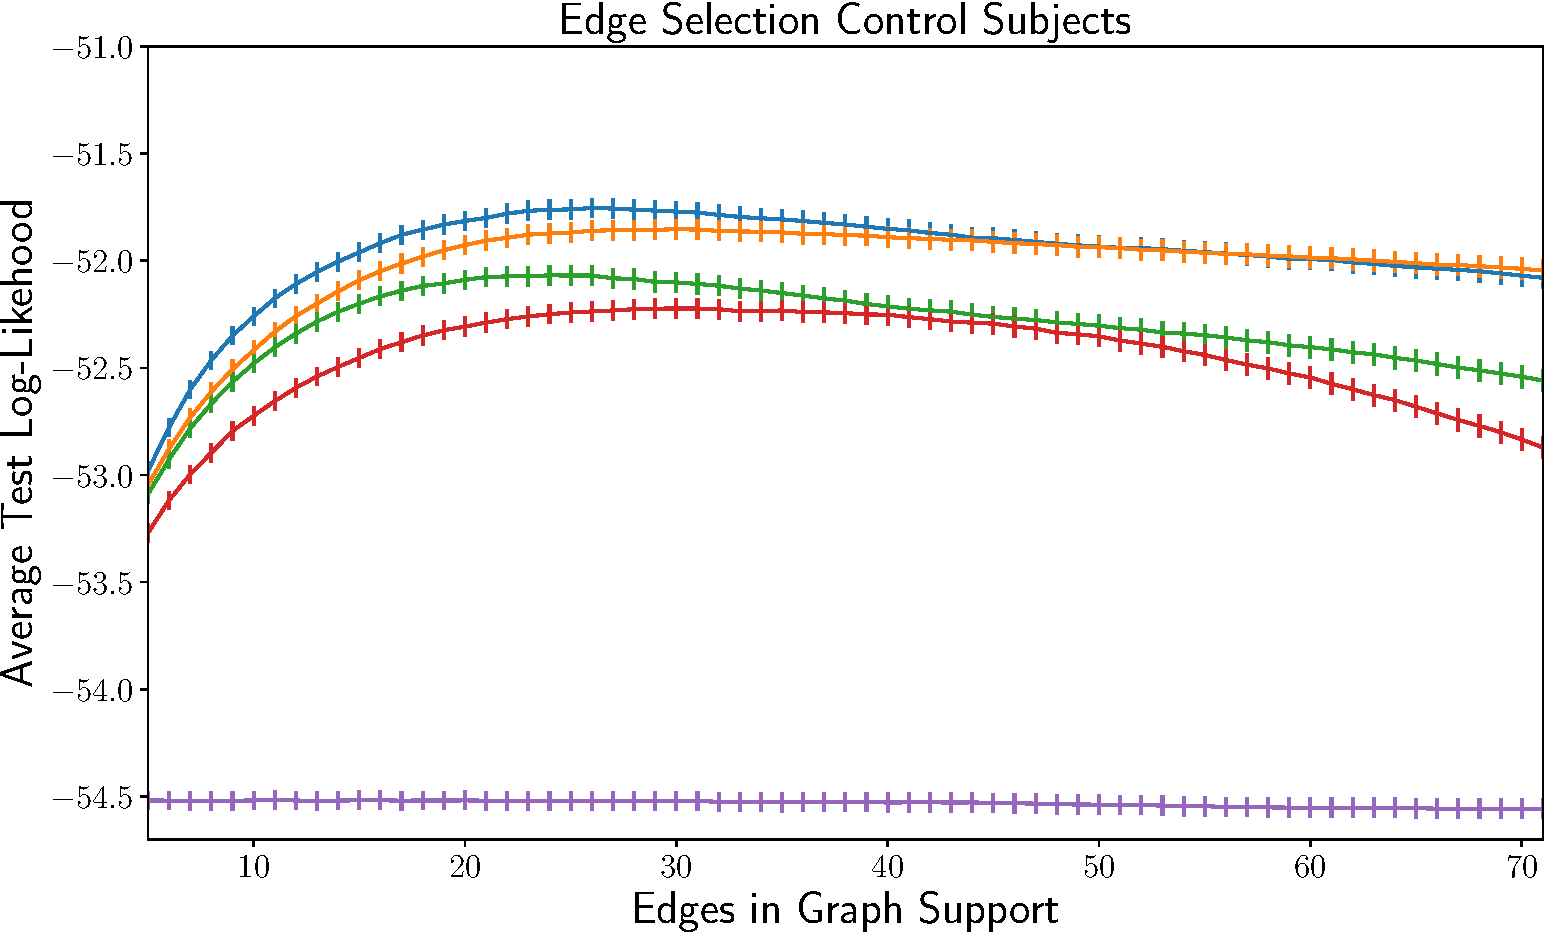
\includegraphics[width=1\textwidth,keepaspectratio]{img/New_ABIDE_Control_nsamps_35_repetitions_1479_errobar_1-crop}
      \end{figure}
    \end{column}
  \end{columns}
\end{frame}
\begin{frame}{Experiments (cont'd)}
  \scalebox{0.7}{
  \begin{tabular}{ |c|c|c|c|c| }
 \hline
  			  & Gene BRCA & Gene COAD & ABIDE Control & ABIDE Autistic \\ \hline
 Graph Lasso  & $0.25\pm .003$    & $0.34\pm 0.004$    & $0.21 \pm .003$ &$\bm{0.21 \pm .003}$\\
 Ledoit-Wolfe &$0.12\pm 0.002$  & $0.15 \pm 0.003$ 		&$0.13 \pm .003$&$0.13 \pm .003$\\
 Bdgraph     & $0.07 \pm 0.002$ & $0.08 \pm 0.002 $ & $N/A$ & $N/A$ \\
 DeepGraph  &$\bm{0.48 \pm 0.004}$   & $\bm{0.57 \pm 0.005}$&$\bm{0.23 \pm .004}$&$0.17 \pm .003$\\
 DeepGraph +Permute & $0.42 \pm 0.003  $  &     $0.52 \pm 0.006$&$0.19\pm .004 $&$0.14 \pm .004$\\
 \hline
\end{tabular}
}
\end{frame}
\section{Conclusion}
\begin{frame}{Questions}
  \begin{center}
    \Huge{Questions?}
  \end{center}
  \begin{figure}
    \centering
    
\includegraphics[width=0.5\textwidth, height=1.0\textheight, keepaspectratio]{img/walter.jpg}
  \end{figure}
\end{frame}


\begin{frame}[allowframebreaks]
        \frametitle{References}
        \bibliographystyle{chicago}
        \bibliography{learning_graphical_models}
\end{frame}
\end{document}

%%% Local Variables:
%%% mode: latex
%%% TeX-master: t
%%% End:
